%%%%%%%%%%%%%%%%%%%%%%%%%%%%%%%%%%%%%%%%%%%%%%%%%%%%%%%%%%%%%%%%%%%%%%%%
%    INSTITUTE OF PHYSICS PUBLISHING                                   %
%                                                                      %
%   `Preparing an article for publication in an Institute of Physics   %
%    Publishing journal using LaTeX'                                   %
%                                                                      %
%    LaTeX source code `ioplau2e.tex' used to generate `author         %
%    guidelines', the documentation explaining and demonstrating use   %
%    of the Institute of Physics Publishing LaTeX preprint files       %
%    `iopart.cls, iopart12.clo and iopart10.clo'.                      %
%                                                                      %
%    `ioplau2e.tex' itself uses LaTeX with `iopart.cls'                %
%                                                                      %
%%%%%%%%%%%%%%%%%%%%%%%%%%%%%%%%%%
%
%
% First we have a character check
%
% ! exclamation mark    " double quote  
% # hash                ` opening quote (grave)
% & ampersand           ' closing quote (acute)
% $ dollar              % percent       
% ( open parenthesis    ) close paren.  
% - hyphen              = equals sign
% | vertical bar        ~ tilde         
% @ at sign             _ underscore
% { open curly brace    } close curly   
% [ open square         ] close square bracket
% + plus sign           ; semi-colon    
% * asterisk            : colon
% < open angle bracket  > close angle   
% , comma               . full stop
% ? question mark       / forward slash 
% \ backslash           ^ circumflex
%
% ABCDEFGHIJKLMNOPQRSTUVWXYZ 
% abcdefghijklmnopqrstuvwxyz 
% 1234567890
%
%%%%%%%%%%%%%%%%%%%%%%%%%%%%%%%%%%%%%%%%%%%%%%%%%%%%%%%%%%%%%%%%%%%
%
\documentclass[12pt]{iopart}
%Uncomment next line if AMS fonts required
%\usepackage{iopams} 
\usepackage{graphicx}
\usepackage[tight,footnotesize]{subfigure}
\usepackage{algorithm} 
\usepackage{algpseudocode}
\algblock{Input}{EndInput}
\algnotext{EndInput}
\algblock{Output}{EndOutput}
\algnotext{EndOutput}
\newcommand{\Desc}[2]{\State \makebox[2em][l]{#1}#2}
\bibliographystyle{iopart-num}

\begin{document}

\title[An Embedded Visualization Method through Temporal Bibliographic Analysis]{An Embedded Visualization Method through Temporal Bibliographic Analysis}

\author{Yan WANG$^{1,*}$, Mingyu SUN$^1$, Ning HU$^1$, Sentao LIU$^1$, Juncheng SI$^1$}

\address{$^1$ State Grid Shandong DongYing Electric Power Company, DongYing 257091, Shandong Province, China}
\ead{$^*$ zdhkj2019@163.com}
\vspace{10pt}
%\begin{indented}
%\item[]June 2019
%\end{indented}

\begin{abstract}
Visual analytics play an important role in understanding complex datasets, e.g. the bibliographic data set. Word clouds, which use a compact visual form of words, have been used widely to provide the content overview of a set of documents, especially the hot topic trends. In this paper, we proposed a visualization method that embedding the temporal patterns along the word to visually illustrate the hot topic evolution. 
\end{abstract}

%\keyword{bibliographic dataset; word cloud; topic modeling; text visualization;}

%
% Uncomment for keywords
%\vspace{2pc}
%\noindent{\it Keywords}: XXXXXX, YYYYYYYY, ZZZZZZZZZ
%
% Uncomment for Submitted to journal title message
%\submitto{\JPA}
%
% Uncomment if a separate title page is required
%\maketitle
% 
% For two-column output uncomment the next line and choose [10pt] rather than [12pt] in the \documentclass declaration
%\ioptwocol
%



\section{Introduction}

In recent years, word clouds (or tag clouds), which use a compact visual form of words, have been used widely to provide the content overview of a set of documents, e.g. the bibliographic data set. How to provide a pleasing summarization for a huge text data has thus become an important research topic in information visualization. Word clouds are text-based visual representations that display word significance in terms of popularity and importance by using different font sizes and colors. Existing efforts in producing effective tag clouds have achieved certain success especially in addressing many aesthetic issues. However, existing tag clouds are inadequate in portraying temporal content evolution of a set of bibliography documents. For example, to understand how a hot research topic have varied during the last decade could be a difficult task if we just visualize the bibliography collections one by one using tag clouds. A simple animation between different tag clouds at different time points would be inadequate to preserve the context for effectively tracking the evolution of the content to find the sequential patterns or correlations.

To facilitate the understanding of temporal content evolution in a set of bibliography documents, we propose a visualization method that embedding the temporal patterns along the word to visually illustrate the hot topic evolution.

\section{Related Work}

We review previous work related to word cloud visualization and temporal word clouds.

\subsection{Word Cloud Visualization}

A word cloud, also known as a tag cloud, is a visual representation of text data that has been used on the web since 1997\cite{Viegas:2008ew}. A word cloud encodes the frequency of words of a given text into font size and color\cite{Rivadeneira:2007ge}, and spatially arranges the words on the canvas. Standard word cloud visualizations use a rectangular line-by-line layout, where the words may be sorted alphabetically or by their importance. To produce more compact and aesthetic visualizations, a large family of alternative layout methods have been proposed\cite{LocarekJunge:2010cy, kaser2007tag, Seifert:ha, Strobelt:2012co, Viegas:km, Wang:2018ji}. Among them, the most well-known algorithm is EdWordle\cite{Wang:2018ji}, a method for consistently editing word clouds, which allows users to move and edit words while preserving the neighborhoods of other words. However, such enhancements still do not capture the relationship between words, let alone the temporal coherence of time-varying text data. Therefore, a variety of temporal word cloud generation methods have been proposed in recent years.

\subsection{Temporal Word Clouds}

Given a time-varying set of words, temporal word clouds attempt to visualize temporal trends while preserving temporal coherence. Collins et al. \cite{Collins:cn} introduce Parallel TagClouds that combine parallel coordinates and traditional word clouds, where the words of each document are distributed along each coordinate axis. Lee et al. \cite{BongshinLee:gz} present the Sparkclouds that visualize trends between multiple word clouds by integrating spark lines into a word cloud. Both methods perform well in the visualization of trends, with the Sparkclouds being the better one in terms of scalability. Cui et al. \cite{Cui:jj} combine a trend chart and multiple word clouds together to illustrate temporal changes of the underlying data. By combining multidimensional scaling and force-directed layout, this method can create semantic and stable word clouds over time. Recently, Chi et al. \cite{Chi:gr} propose a morphable word clouds, where a sequence of spatial shapes is specified as a boundary for a set of time-varying word clouds. By using rigid body dynamics, they arrange words within the given shape sequence so that temporal changes are encoded by both the shapes and the content of the word clouds. In this paper, we proposed an embedded temporal visualization method to present the temporal patterns in the text.

\section{Proposed Technique}

\subsection{Motivation}

Models of bibliographic data need to consider many kinds of information. Articles are usually accompanied by metadata such as authors, publication data, categories and time\cite{Lim2016}. Bibliographic analysis considers the author’s research areas, the citation network and the paper content among other things, which can be combined into a topic model that produces a bibliographic model of authors, topics and documents. In this paper, We propose a novel and efficient inference visualization algorithm to explore the constantly change of the hot topics.


\subsection{System Overview}

To facilitate generation of visual output at all three levels, a flexible mapping strategy is required. Such a strategy has been manifested as the so-called visualization pipeline. The visualization pipeline leveraged in this paper is proposed by Santos and Brodlie\cite{dosSantos:2004ck}, which consists of the three steps: filtering, mapping and rendering (see Figure \ref{fig:pipeline}).

\begin{figure}
    \centering
    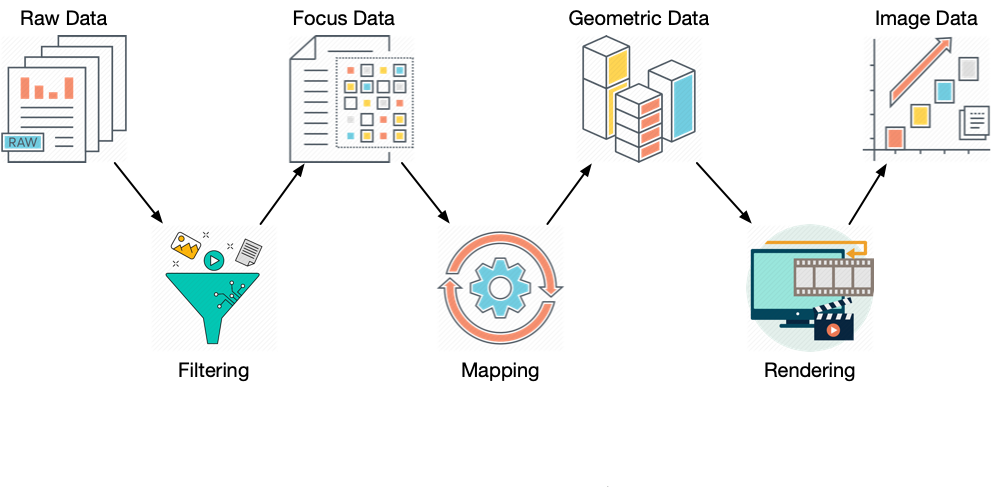
\includegraphics[width=.95\textwidth]{images/pipeline.png}
    \caption{Visualization Pipeline}
    \label{fig:pipeline}
\end{figure}

The filtering step prepares the raw input data for processing through the remaining steps of the pipeline. This is done with respect to the given analysis task and includes not only selection of relevant data but also operations for data enrichment or data reduction, interpolation, data cleansing, grouping, dimension reduction, and others. 

Literally, the mapping step maps the prepared data to appropriate visual variables. This is the most crucial step as it largely influences the expressiveness and effectiveness of the resulting visual representation. 

Finally, the rendering step generates actual images from the previously computed geometry and visual attributes. This general pipeline model is the basis for many visualization systems.

\section{Temporal Display Design}
\label{sec:tdd}

The bibliography raw data usually is collected in plain text files, and organized by a standard rule, such as BibTex, EndNote etc. In this paper, we use the IEEE VIS conference series data\cite{Isenberg:2016ika} from 1990 to 2016 to illustrate the usage of our method. The data used in our experiments contains IEEE VIS publications, i.e., InfoVis, SciVis, VAST, or Vis. Each record consists of 11 fields, including conference type, publication year, paper title, DOI, abstract, author names, and references (inside this dataset only). In the purpose of exploring research topic, only some fields are involved in the proposed method, which contains the topic features and temporal features. Specifically, the topic features will be extracted from these fields, which are paper title, abstract, and full text if available. The temporal features will be aggregated by the time granularity, which is the 'year' data field in this case. 

\subsection{Data Processing}

The raw data contains topic features and temporal features will be filtered into the focus data by the data processing approach. The raw data is composed by records, which could be distinct from each other by some specific notations or punctuation, such as a semicolon or a line break. Let's define the raw data set is $X := \{X^{(1)},X^{(2)},...,X^{(n)}\}$, where the $n$ is the number of records contained in the raw data, and the $X^{(i)}$ means the $i$th record in $X$ with $1 \leq i \leq n$. 

To show the temporal visualization of the bibliography data set, both the words variable and the times variable should be considered in the data processing approach. To achieve a better visualization presentation with clarity and concision, the method proposed in this paper gives a general pipeline to declare the details of the data processing. 

An ignored word list and a merged word list should be initialized before the data processing approach, and will be continuous updated during the data exploring activity. 

The ignored word list contains frequently used words (such as and, the, because, and so on) or words that you do not want indexed, which will be excluded from the result. The data processing program comes with a default set of ignored words that you can modify as needed. The ignored word list could be defined as $ P := \{P_1,P_2,...,P_m\} $, where $P_i$ with $1 \leq i \leq m$ means a single word will be ignored. 

The merged word list is composed by several word groups, each group contains the words which is a synonym for each other. The merged word list is defined as $ M := \{ M^{(1)}, M^{(2)},...,M^{(n)} \} $, where $M^{(i)}$ with $1 \leq i \leq n$ means the $i$th merged word group. The merged word group is an order-sensitive sequence, which is defined as $M^{(i)} := \{ M_1^{(i)},M_2^{(i)},...,M_m^{(i)}\}$, and all the words in the same merged word group will be merged into the first word in the sequence. The merged word list can be initialized by several approaches. One of the most leveraged method is the word distance algorithm, such as the Levenshtein algorithm, which is a string metric for measuring difference between two sequences. Informally, the Levenshtein distance between two words is the minimum number of single-character edits (i.e. insertions, deletions or substitutions) required to change one word into the other. But the word distance algorithm should be applied under supervision. For example, the words "universe" and "university" are quit similar but with very different meaning.

Given the ignored word list and the merged word list, the raw data processing program could be leveraged to produce the focus data set, which is defined as $R := \{R_1,R_2,...,R_n\}$, where $R_i := \{word, weight, seq \}$ and $seq := [\{t_1,v_1\},...,\{t_n,v_n\}]$. Considering the visual dimension, the focus data set only contains the $n$ records of the whole data set, following the rule of sorting the records in descending order by the weight variable of each record. The raw data processing program is briefly described in a pseudo code block, as is shown in algorithm \ref{alg:data-process}.

\begin{algorithm}
	\caption{Data Processing Algorithm}
	\label{alg:data-process}
	\begin{algorithmic}[1]
	
\Input
\Desc{X}{raw data set}
\Desc{P}{ignored word list}
\Desc{M}{merged word list}
\Desc{n}{return the top \textit{n} records}
\EndInput
\Output
\Desc{R}{$ R := \{R_1,R_2,...,R_n\}$} 
\Comment {where $R_i := \{word, weight, seq \}$} \\
\Comment {$seq := [\{t_1,v_1\},...,\{t_n,v_n\}]$}
\EndOutput

\Procedure{DataProcess}{$X, P, M, n$}
\State $t_{min} \gets \Call{MinYear}{X}$
\State $t_{max} \gets \Call{MaxYear}{X}$
\State $ry \gets t_{max} - t_{min} + 1$
\Comment{ry: the time range in years}
\State $R = \emptyset$
\For { $\forall X^{(i)} \in X$}
	\For { $\forall w, t \in X^{(i)}$} 
		\Comment{w is the word in text mode, t is the time variable}
		\If{$ w \in P $}
		\State{\textbf{continue}}
		\EndIf
		\For{$\forall M^{(i)} \in M$}
			\If{$ w \in M^{(i)} $}
				\State{$w \gets M^{(i)}_0$} 
				\Comment{$M^{(i)}_0$ is the replacement in the group $M^{(i)}$}
				\State $found \gets false $
				\For{$\forall R_i \in R$}
					\If{$\exists R_i[word] = w$}
						\State $found \gets true $
						\State $R_i[weight] \gets R_i[weight] + 1$
						\State $j \gets t-t_{min}$
						\State $R_i[seq][j] \gets R_i[seq][j] + 1$
					\EndIf
					
				\EndFor
				\If{$ not found$}
				\State $word \gets w, weight \gets 1, seq \gets \Call{Array}{ry}$
				
				\State $seq[t-t_{min}] \gets \{t,1\}$
				\State $ R \gets R \cup \{word,weight,seq\} $
				\EndIf
			\EndIf
		\EndFor
	\EndFor
\EndFor
\State \Call{Sort}{R}
\Comment{Sort R in descending order by weight }
\State \textbf{Return} $R[1,...,n]$ 
\Comment{Only the top $n$ records are needed}
\EndProcedure

\end{algorithmic}
\end{algorithm}


\subsection{Data Mapping}

The mapping from focus data to geometric data is the core of our method. Compared to traditional word cloud visualization algorithm, e.g. the Wordle layout algorithm, our method has considered the relevant temporal patterns additionally.

The word layout algorithm is revealed in the pseudo code as shown in algorithm \ref{alg:wordlayout}. The whole process of the algorithm is similar to the Wordle layout algorithm, but with one bit improvement, which is the placement of the underline pattern bar under the word area before the detection of the intersections. For each word in the focus data, the algorithm gives the dimension of the word and the relevance font size when there is no intersections with any previously placed words.

The temporal pattern related to each word is encoded into the underline pattern bar, which is split joint by a rectangle sequence filled with a correlated color. There is a one-to-one relationship between the temporal pattern and the rectangle sequence, and the numeric value in the temporal pattern is encoded to a color.

\begin{algorithm}
\caption{Word Layout Algorithm}
\label{alg:wordlayout}
\begin{algorithmic}[1]
\Input
\Desc{R}{$ R := \{R_1,R_2,...,R_n\}$}\\
\Comment {$R_i := \{word, weight, seq \}$} \\
\Comment {$seq := [\{t_1,v_1\},...,\{t_n,v_n\}]$}
\EndInput
\Output
\Desc{R}{$ R := \{R_1,R_2,...,R_n\}$}\\
\Comment {$R_i := \{word, weight, seq, size, d, colors\}$} \\
\Comment {$d := \{x,y,w,h\}$}
\EndOutput

\Procedure{WordLayout}{$R$}
\For{$\forall R_i \in R$}
\State $ R_i[size] \gets \Call{FontSizeScale}{R_i[weight]}$
\State $ R_i[colors] \gets \Call{ColorScale}{R_i[seq]}$
\Repeat
\State $ \Call{MoveAlongSpiralPath}{R_i[word]}$
\State $ \Call{PlacementStrategy}{R_i[word]}$
\State $ \Call{PlaceUnderlinePatternBar}{R_i[word]}$
\Until{no intersection detected}

\Return $R$
\EndFor

\EndProcedure
\end{algorithmic}
\end{algorithm}

\subsection{Visualization Result}

To demonstrate the proposed visualization method in this paper, an evaluation experiment is developed base on the IEEE VIS conference series data (as mentioned in section \ref{sec:tdd}). The experiment is implemented by JavaScript program language, and  exhibited in the chrome browser. The data mapping part of the algorithm leverages the "Canvas" technique to perform the intersection detection during the word layout phase. The final visualization effect is achieved by the "SVG" specification provided by a third-party library named $D^3$\cite{Bostock:da}. A final visual snapshot of the system is shown in the figure \ref{fig:twc}. By utilizing the system, a researcher could have a good understanding what aspects to consider when selecting a topic for the research paper. 

\begin{figure}
	\centering
	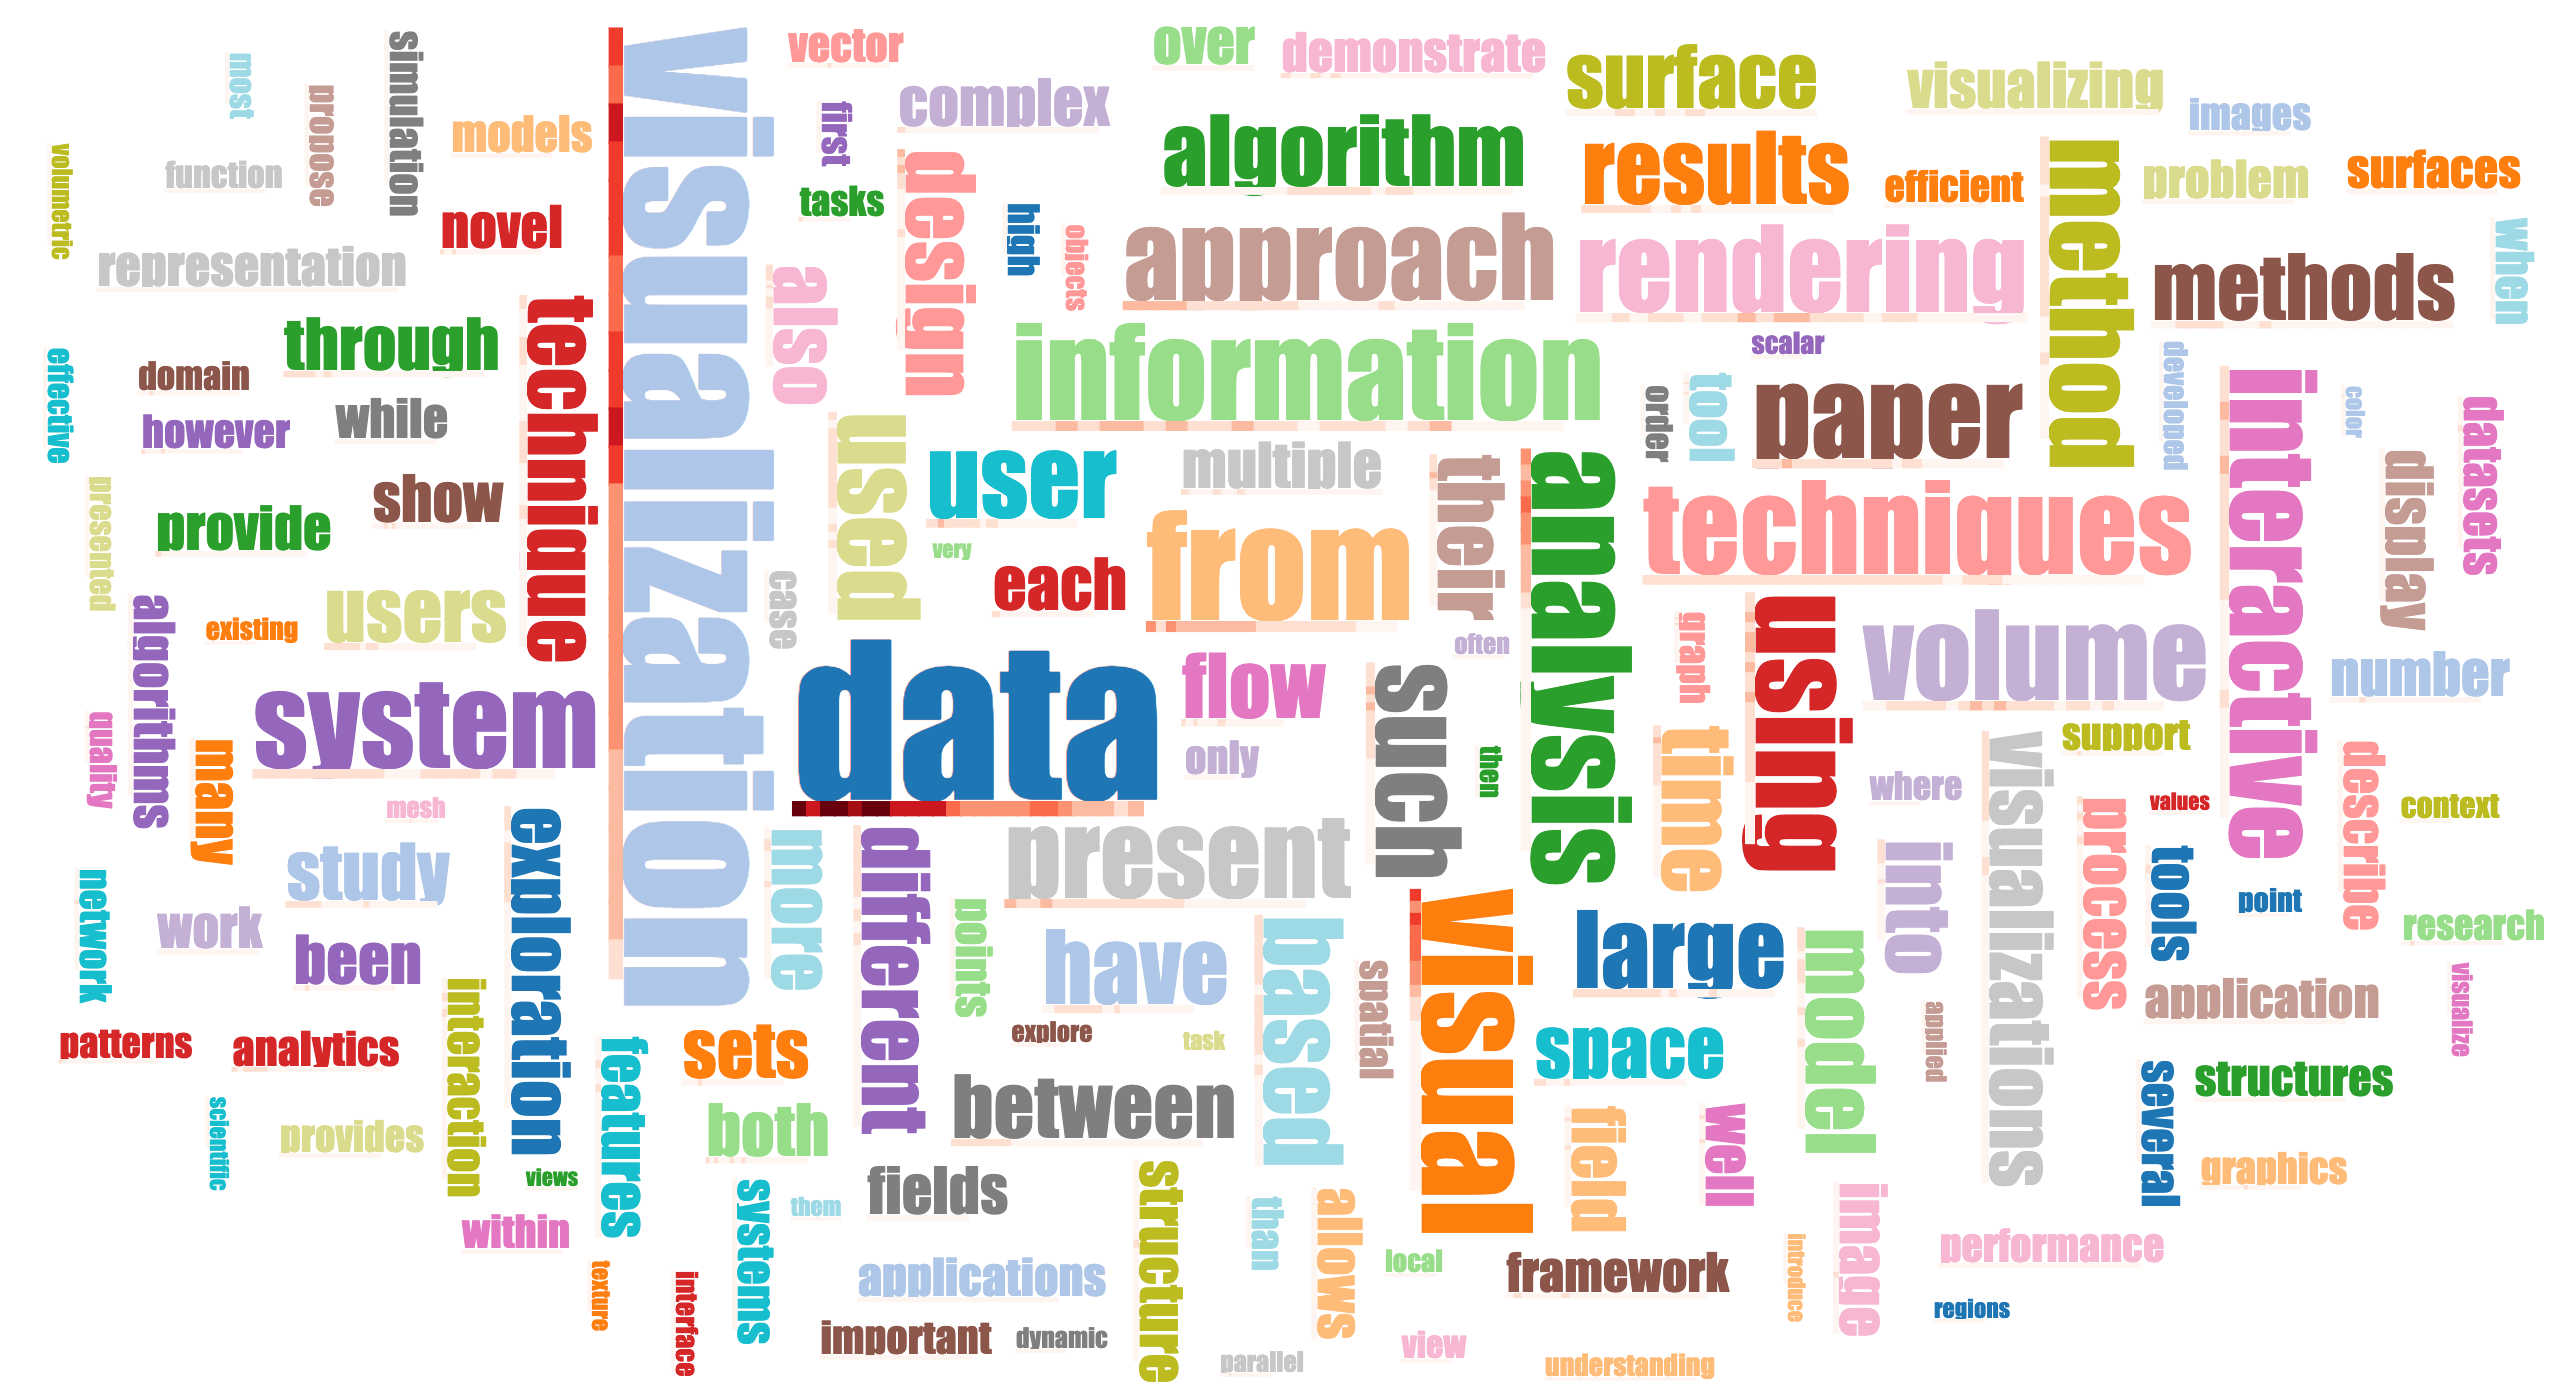
\includegraphics[width=.95\textwidth]{images/wordcloud}
	\caption{Temporal Word Cloud}
	\label{fig:twc}
\end{figure}

\section{Conclusion}

In this paper, we proposed an embedded visualization method to facilitate the understanding of temporal content evolution in a set of bibliography documents by visually illustrating the hot topic evolution. A system is developed and demonstrated to evaluate the method, which given a very positive feedback. But the current version of the system is lacking of an interactive user interface, which causes a bad performance in parameter adjustment. In the future work, an interactive control panel will be mounted on the interface, which will improve the user experience.

\section{Acknowledgements}

This work was supported by "Research on Lightweight Active Immune Technology for Electric Power Supervisory Control System", a science and technology project of State Grid Co.,Ltd in 2019.

\section{References}
\bibliography{references}

\end{document}

